\documentclass[twocolumn,a4paper,dvipdfmx]{ieicejsp}
\usepackage[T1]{fontenc}
\usepackage{lmodern}
\usepackage{textcomp}
\usepackage{latexsym}
\usepackage{float}
\usepackage{graphicx}
\usepackage{amsmath, amssymb}
\usepackage{bm}
\usepackage{upgreek}
\usepackage{caption}
\usepackage{booktabs}
\usepackage{multirow}
\usepackage{url}

\captionsetup{font=small}
\DeclareMathOperator*{\argmax}{arg\,max}

\title{
    {\bf 粒度可変物体アノテーションにおけるSigLIPのシグモイド確信度，\\YOLOとVLMのスコアの比較およびWordNetの同じ深さの語彙の検証}
    {\normalsize \\ Sigmoid Confidence of SigLIP, Score Comparison between YOLO and VLM, and Same-Depth WordNet Vocabulary for Adjustable-Granularity Object Annotation}
}
\author{
    著者名 \\ Author Name
}
\affliate{%
    所属機関名 \\
    Affiliation \\
}

\begin{document}
\maketitle

\begin{abstract}
本稿では，検出と命名を分離した粒度可変物体アノテーションにおいて，現在の構成（CLIP-ViT-B/32とソフトマックス，COCOの80クラスを深さ0とするハイブリッド構成）に対し，3つの変更を加えた構成を比較する．
第一の変更は，視覚言語モデル（Vision-Language Model，VLM）をSigLIPに置き換え，候補語彙の中で正規化するソフトマックスの代わりに語ごとに独立なシグモイドで確信度を計算することである．
第二の変更は，YOLOの検出ボックスのクロップに対するVLMの最大確信度がYOLOの検出スコアを上回る場合にVLMの語を深さ0とすることである．
第三の変更は，YOLOを再学習せずにCOCO外の語へ対応するため，WordNetにおいてCOCOのカテゴリと同じ深さにある語彙を深さ0の候補とすることである．
COCO 2017 Validationの重複しない検証用・テスト用の分割とLVISの細かい粒度の正解を用いた評価により，以下を確認した．
シグモイドは，深さ0が誤った枝における最深段の確信度の識別性能（AUROC）をハイブリッド構成で0.418から0.617へ改善する一方，深さ0が正しい場合の深さ1の正誤の識別ではソフトマックスに劣る（0.762に対し0.644）．
スコアの比較による切替は，ソフトマックスではCOCOのTop-1正解率を0.969から0.936（CLIP）および0.858（SigLIP）へ低下させ，シグモイドでは切替がほとんど生じない．
WordNetの同じ深さの語彙（681語）を用いると，COCO外の物体の深さ0が正しい上位語となる割合は0から3.8\%に増えるが，COCOのTop-1正解率は0.945へ低下する．
\end{abstract}

\noindent
{\bf キーワード：}SigLIP，シグモイド，ソフトマックス，確信度，WordNet，オープンボキャブラリ物体アノテーション

\section{はじめに}
検出と命名を分離した粒度可変物体アノテーションでは，Detection Transformer（DETR）\cite{ref_DETR}またはYOLO\cite{ref_YOLO}で検出した領域のクロップに対し，Contrastive Language-Image Pre-training（CLIP）\cite{ref_CLIP}のゼロショット分類で深さ0の単語を決め，WordNet\cite{ref_WordNet}の下位語を候補語彙として同じクロップの分類を繰り返す．
現在の構成には3つの課題がある．
第一に，CLIPの確信度は候補語彙の中で正規化するソフトマックスで計算されるため，候補語彙に正しい語が含まれない場合でも，候補の中で相対的に最もよい語に高い確信度が与えられる．
この結果，深さ0が誤ったまま下位語へ展開された枝において，深い段階の確信度で誤りを検出できない．
第二に，COCO\cite{ref_COCO}の80クラスで学習したYOLOを深さ0に用いるハイブリッド構成は，80クラスの範囲では高い精度を示すが，YOLOの予測を覆す規則はCOCO外の22語の確信度に対する閾値に限られる．
第三に，COCO外の22語は人手で選んだ語であり，YOLOを再学習せずにCOCO外の語彙へ体系的に対応する方法がない．

本稿では，これらの課題に対応する3つの変更として，シグモイドで確信度を計算するSigLIP\cite{ref_SigLIP}への置き換え，YOLOとVLMのスコアの比較による深さ0の決定，およびWordNetにおいてCOCOのカテゴリと同じ深さにある語彙による深さ0の候補を導入し，現在の構成と同一の分割・評価指標で比較する．

\section{比較する構成}
\subsection{ソフトマックスとシグモイドによる確信度}
クロップ$ X $の画像特徴を$ {\mathbf x} \in {\mathbb R}^{1 \times D} $，候補語彙$ {\mathbb V} $に含まれる語$ v $のプロンプト「a photo of a $ v $」のテキスト特徴を$ {\mathbf w}_v \in {\mathbb R}^{1 \times D} $とし，いずれもL2正規化されているとする．
VLMは語$ v $のロジットを(\ref{eq_logit})で計算する．

\begin{equation}
    l_v = t \, {\mathbf x} {\mathbf w}_v^{\top} + b
    \label{eq_logit}
\end{equation}

\noindent
ここで$ t > 0 $は学習済みの温度，$ b $は学習済みのバイアスであり，CLIPでは$ b = 0 $である．
現在の構成は確信度を(\ref{eq_softmax})のソフトマックスで計算し，SigLIPの学習時の目的関数と同じ形のシグモイドでは(\ref{eq_sigmoid})で計算する．

\begin{align}
    p_v^{\mathrm{soft}} &= \frac{\exp(l_v)}{\sum_{u \in {\mathbb V}} \exp(l_u)}
    \label{eq_softmax} \\
    p_v^{\mathrm{sig}} &= \frac{1}{1 + \exp(-l_v)}
    \label{eq_sigmoid}
\end{align}

\noindent
$ p_v^{\mathrm{soft}} $は候補語彙の和が1となるため，候補語彙が1語の段階では必ず1となる．
一方，$ p_v^{\mathrm{sig}} $は他の語に依存せず，画像と語の対応の度合いを絶対的に表す．
両者の$ \argmax $は一致するため，各段階で選ばれる語は同じであり，確信度のみが異なる．
深さ$ d $の累積確信度$ c^{(d)} = \prod_{j=0}^{d} p^{(j)} $が閾値$ \tau $を下回る前の深さで細分化を止め，$ c^{(0)} < \tau $の場合は棄却する停止規則を用いる．
ここで$ p^{(j)} $は深さ$ j $で選ばれた語の確信度であり，ハイブリッド構成の$ p^{(0)} $はYOLOの検出スコアである．
VLMはCLIP-ViT-B/32と，同程度の規模のSigLIP-ViT-B/16（WebLIで学習）を用いる．
モデルの変更による効果と正規化関数の変更による効果を分けるため，CLIPとソフトマックス，SigLIPとソフトマックス，SigLIPとシグモイドの3つの組を比較する．

\subsection{YOLOとVLMのスコアの比較による深さ0の決定}
YOLOが出力した語を$ v_{\mathrm{Y}} $，検出スコアを$ s_{\mathrm{Y}} $とし，同じボックスのクロップに対するVLMの深さ0の候補語彙$ {\mathbb V}_0 $上の最大確信度の語を$ v_{\mathrm{V}} = \argmax_{v \in {\mathbb V}_0} p_v $とする．
スコアの比較による構成（以下，hybrid\_cmp）は深さ0の語$ v^{(0)} $を(\ref{eq_cmp})で決める．

\begin{equation}
    v^{(0)} =
    \begin{cases}
        v_{\mathrm{V}} & \mathrm{if} \ p_{v_{\mathrm{V}}} > s_{\mathrm{Y}}, \\
        v_{\mathrm{Y}} & \mathrm{otherwise}
    \end{cases}
    \label{eq_cmp}
\end{equation}

\noindent
比較対象は，YOLOの語をそのまま用いる構成（hybrid）と，COCOの80クラスとCOCO外の22語からなる102語上の$ v_{\mathrm{V}} $がCOCO外の語であり，かつ$ p_{v_{\mathrm{V}}} \geq 0.5 $の場合のみ$ v_{\mathrm{V}} $を用いる現在の構成（hybrid\_switch\_c0.5）である．
hybrid\_cmpでは$ {\mathbb V}_0 $をCOCOの80クラスとする．

\subsection{WordNetの同じ深さの語彙}
WordNetの根からの深さは上位語の経路によって大きく異なり，例えばdogは深さ8と13の経路を持つ．
このため，木全体での絶対的な深さを揃えても粒度は揃わない．
そこで，COCOのカテゴリのSynset $ c $ごとに，最長の上位語の経路で$ k $段上の祖先$ a_k(c) $をとり，$ a_k(c) $からちょうど$ k $段下にあるSynsetの集合を，$ c $と同じ深さの語の集合とする．
深さ0の候補語彙を(\ref{eq_wn_vocab})で定義する．

\begin{equation}
    {\mathbb V}_0^{(k)} = {\mathbb C} \cup \Bigl\{ s \in \bigcup_{c \in {\mathbb C}} {\mathcal H}^{k}\bigl(a_k(c)\bigr) \Bigm| \phi(s) \Bigr\}
    \label{eq_wn_vocab}
\end{equation}

\noindent
ここで$ {\mathbb C} $はCOCOの80クラスのSynsetの集合，$ {\mathcal H}^{k}(a) $は$ a $から$ k $段下の下位語の集合である．
$ \phi(s) $は，$ s $が物理的な実体（physical\_entity.n.01）の下位語であり，$ {\mathbb C} $のいずれかの上位語でも下位語でもなく，SemCor\cite{ref_SemCor}における出現頻度が1以上であることを表す．
例えば$ k = 2 $では，dogの2段上の祖先carnivoreから2段下のwolfやfoxが含まれ，birdより深いpenguinや，birdより浅いanimalは含まれない．
$ k = 2 $の語彙を用い，(\ref{eq_cmp})の$ {\mathbb V}_0 $を$ {\mathbb V}_0^{(2)} $とした構成をhybrid\_cmp\_wn2，DETRの検出に対し$ {\mathbb V}_0^{(2)} $から深さ0を選ぶ構成をproposed\_wn2と呼ぶ．

\section{実験}
\subsection{実験条件}
COCO 2017 Validationの5000枚を重複しない検証用とテスト用に分割する．
検証用はseed 42でサンプリングした500枚（dev500）とLVIS\cite{ref_LVIS}のアノテーションが存在する2604枚（lvis\_dev）であり，テスト用は残りの画像から別にサンプリングした500枚（test500，GTインスタンス3748件）とLVISのアノテーションが存在する2148枚（lvis\_test）である．
本稿の結果はすべてテスト用の分割の値であり，$ \tau $はlvis\_devで階層的F値$ hF $が最大となる値を選んだ．
検出スコアの閾値は，評価インスタンス数が近い組である，DETRの$ \theta = 0.5 $（以下，proposed）とYOLO11xの0.25（以下，hybrid）を主に示す．
COCOのGTとIoUが0.5以上で対応した検出について，深さ0のTop-1正解率を評価する．
深さ1以降は，COCOのカテゴリより細かいLVISのSynsetをIoUが0.5以上で対応付けたインスタンス（proposedで489件，hybridで481件）について，COCOのSynsetからLVISのSynsetまでの経路を正解とする階層的適合率$ hP $，再現率$ hR $，F値$ hF $\cite{ref_hF}で評価する．
COCO外の物体の評価には，lvis\_testにおいて，SynsetがCOCOのカテゴリの上位語・下位語でなく，レンマ名もCOCOのカテゴリ名と一致しないLVISのアノテーション（511カテゴリ）に対応し，COCOのGTとは対応しない検出ボックスを用いる．
評価インスタンスはhybridで262件（117カテゴリ），proposedで521件（175カテゴリ）である．
深さ0の語がLVISのSynsetの上位語または自身である割合を，COCO外の物体の正解率とする．

\subsection{ソフトマックスとシグモイドの比較}
表\ref{tab_normalization}と図\ref{fig_auroc}にVLMと正規化関数ごとの結果を示す．
図\ref{fig_auroc}(a)は，test500において深さ0が正しい枝と誤った枝を，最深段の確信度で区別する性能をAUROCで示す．
図\ref{fig_auroc}(b)は，lvis\_testにおいて深さ0が正しいインスタンスの深さ1の正誤を，深さ1の確信度で区別する性能をAUROCで示す．

\begin{table*}[t]
    \centering
    \caption{VLMと正規化関数の比較（テスト用の分割）．Top-1はtest500の深さ0のTop-1正解率，誤枝AUROCは深さ0の正誤を最深段の確信度および累積確信度で区別するAUROC，深さ1はlvis\_testで深さ0が正しいインスタンスの深さ1の正解率と，深さ1の確信度による正誤のAUROC，$ hF $は$ \tau $による停止規則と深さの上限1による停止規則のlvis\_testの階層的F値である．}
    \label{tab_normalization}
    \begin{tabular}{llcccccccc}
        \toprule
        & & & \multicolumn{2}{c}{誤枝AUROC} & \multicolumn{2}{c}{深さ1} & \multicolumn{3}{c}{$ hF $} \\
        \cmidrule(lr){4-5} \cmidrule(lr){6-7} \cmidrule(lr){8-10}
        手法 & VLMと正規化関数 & Top-1 & 最深段 & 累積 & 正解率 & AUROC & $ \tau $ & $ \tau $による停止 & 深さ1まで \\
        \midrule
        \multirow{3}{*}{proposed} & CLIP + ソフトマックス & 0.552 & 0.611 & 0.508 & 0.440 & 0.744 & 0.2 & 0.462 & 0.451 \\
        & SigLIP + ソフトマックス & 0.527 & 0.600 & 0.634 & 0.462 & 0.843 & 0.5 & 0.480 & 0.453 \\
        & SigLIP + シグモイド & 0.527 & 0.715 & 0.633 & 0.462 & 0.587 & $ 10^{-4} $ & 0.450 & 0.453 \\
        \midrule
        \multirow{3}{*}{hybrid} & CLIP + ソフトマックス & 0.969 & 0.418 & 0.430 & 0.407 & 0.762 & 0.3 & 0.647 & 0.648 \\
        & SigLIP + ソフトマックス & 0.969 & 0.480 & 0.483 & 0.405 & 0.780 & 0.3 & 0.648 & 0.648 \\
        & SigLIP + シグモイド & 0.969 & 0.617 & 0.594 & 0.405 & 0.644 & 0.05 & 0.659 & 0.648 \\
        \bottomrule
    \end{tabular}
\end{table*}

\begin{figure}[t]
    \centering
    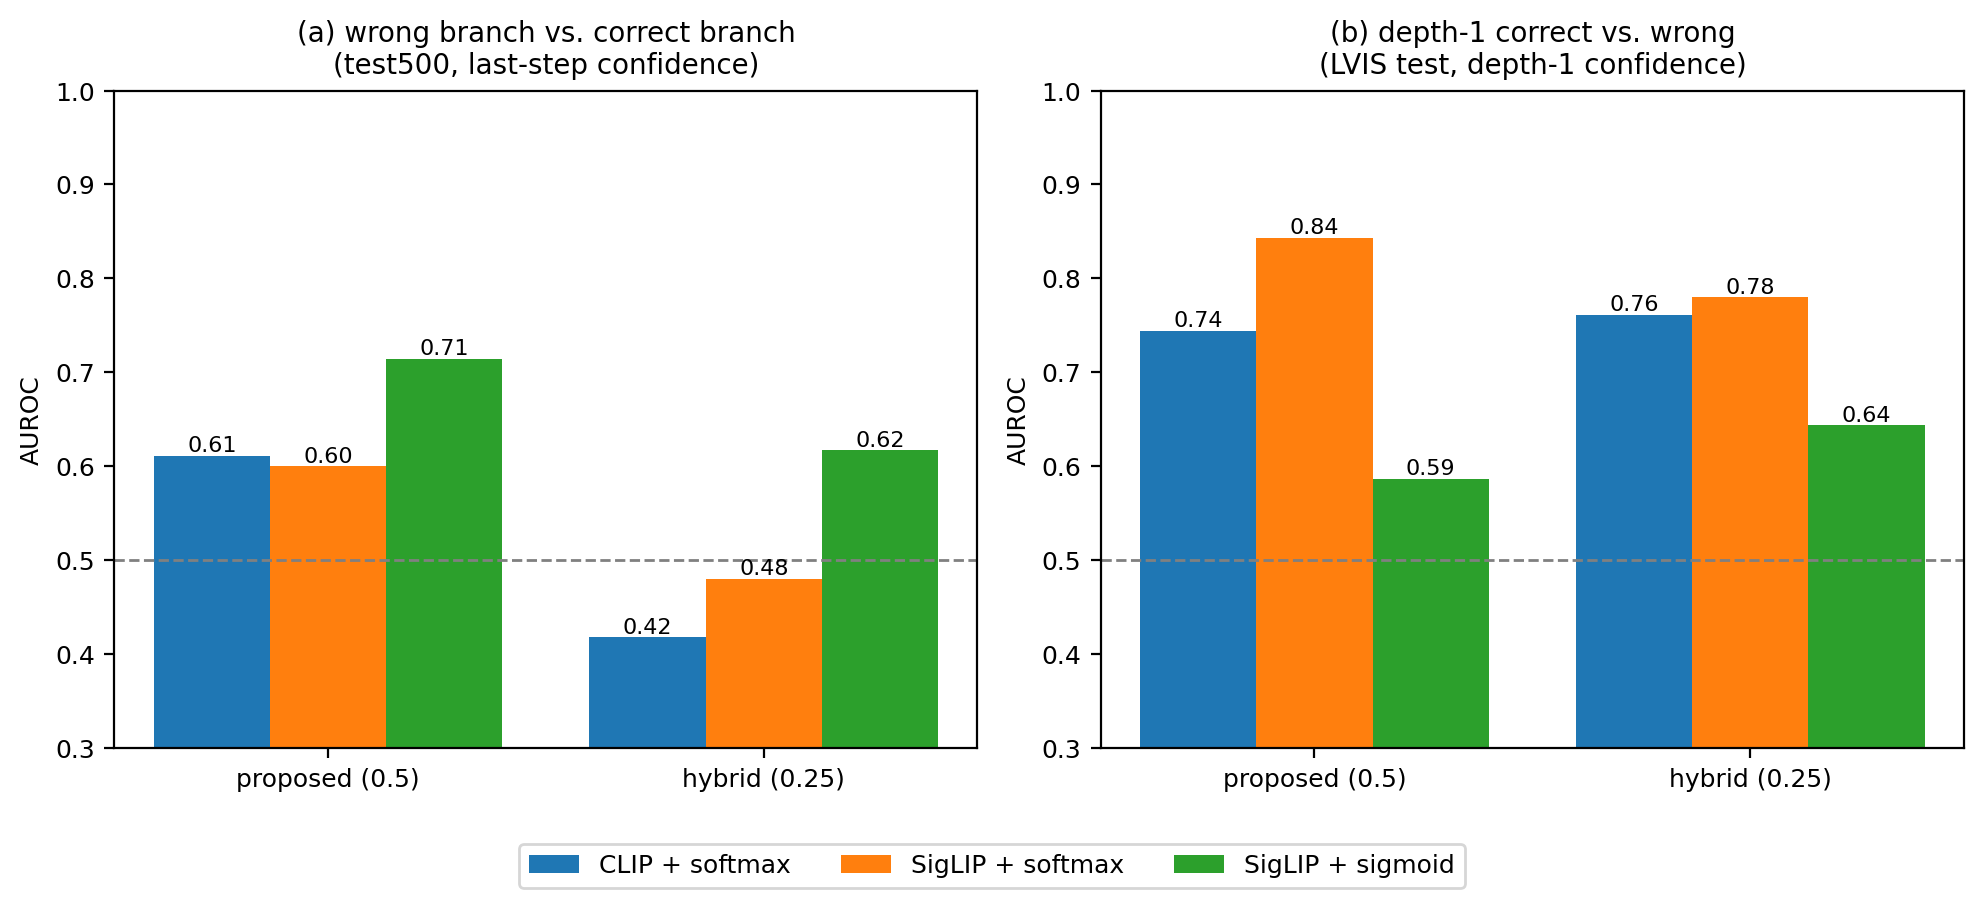
\includegraphics[width=\linewidth]{figures/fig_auroc.png}
    \caption{確信度による正誤の識別性能．(a)はtest500で深さ0が正しい枝と誤った枝を最深段の確信度で区別するAUROC，(b)はlvis\_testで深さ0が正しいインスタンスの深さ1の正誤を深さ1の確信度で区別するAUROCである．破線は偶然の水準0.5である．}
    \label{fig_auroc}
\end{figure}

表\ref{tab_normalization}から，SigLIPのTop-1正解率はproposedでCLIPより0.025低く，hybridでは深さ0がYOLOで決まるため同じである．
図\ref{fig_auroc}(a)から，シグモイドは誤った枝の識別性能を，hybridで0.418から0.617へ，proposedで0.611から0.715へ改善した．
SigLIPにソフトマックスを用いた場合のhybridのAUROCは0.480であり，この改善はモデルの変更ではなく正規化関数の変更によるものである．
ソフトマックスでは，誤った枝の候補語彙に正しい語が含まれなくても候補の中で相対的に最もよい語の確信度が高くなるのに対し，シグモイドでは画像と語の対応が弱い場合に確信度が低くなるためである．
一方，図\ref{fig_auroc}(b)から，深さ0が正しい場合の深さ1の正誤の識別では，ソフトマックスがシグモイドより高いAUROCを示した．
SigLIPでは，ソフトマックスの0.843（proposed）および0.780（hybrid）に対し，シグモイドは0.587および0.644であった．
兄弟の語の中での相対的な比較が必要な深さ1の判断では，候補語彙の中で正規化するソフトマックスが有利である．

図\ref{fig_stopping_scorers}にlvis\_testにおける停止規則の$ hP $と$ hR $の関係を示す．
横軸は階層的再現率$ hR $，縦軸は階層的適合率$ hP $であり，曲線は$ \tau $を変化させた累積確信度による停止規則，四角は深さの上限（0〜3）による停止規則である．
hybridでは，シグモイドの$ \tau = 0.05 $による停止が$ hF = 0.659 $となり，CLIPとソフトマックスの0.647および深さの上限1の0.648をわずかに上回った．
proposedでは，シグモイドの深さ0の確信度が小さいため，$ \tau $を大きくすると多くのインスタンスが深さ0で棄却され，$ hP $の高い領域で他の組より劣った．
シグモイドの深い段階の確信度は0.01以下となる場合が多く，選ばれた$ \tau $は$ 10^{-4} $および0.05と小さい値であった．

\begin{figure}[t]
    \centering
    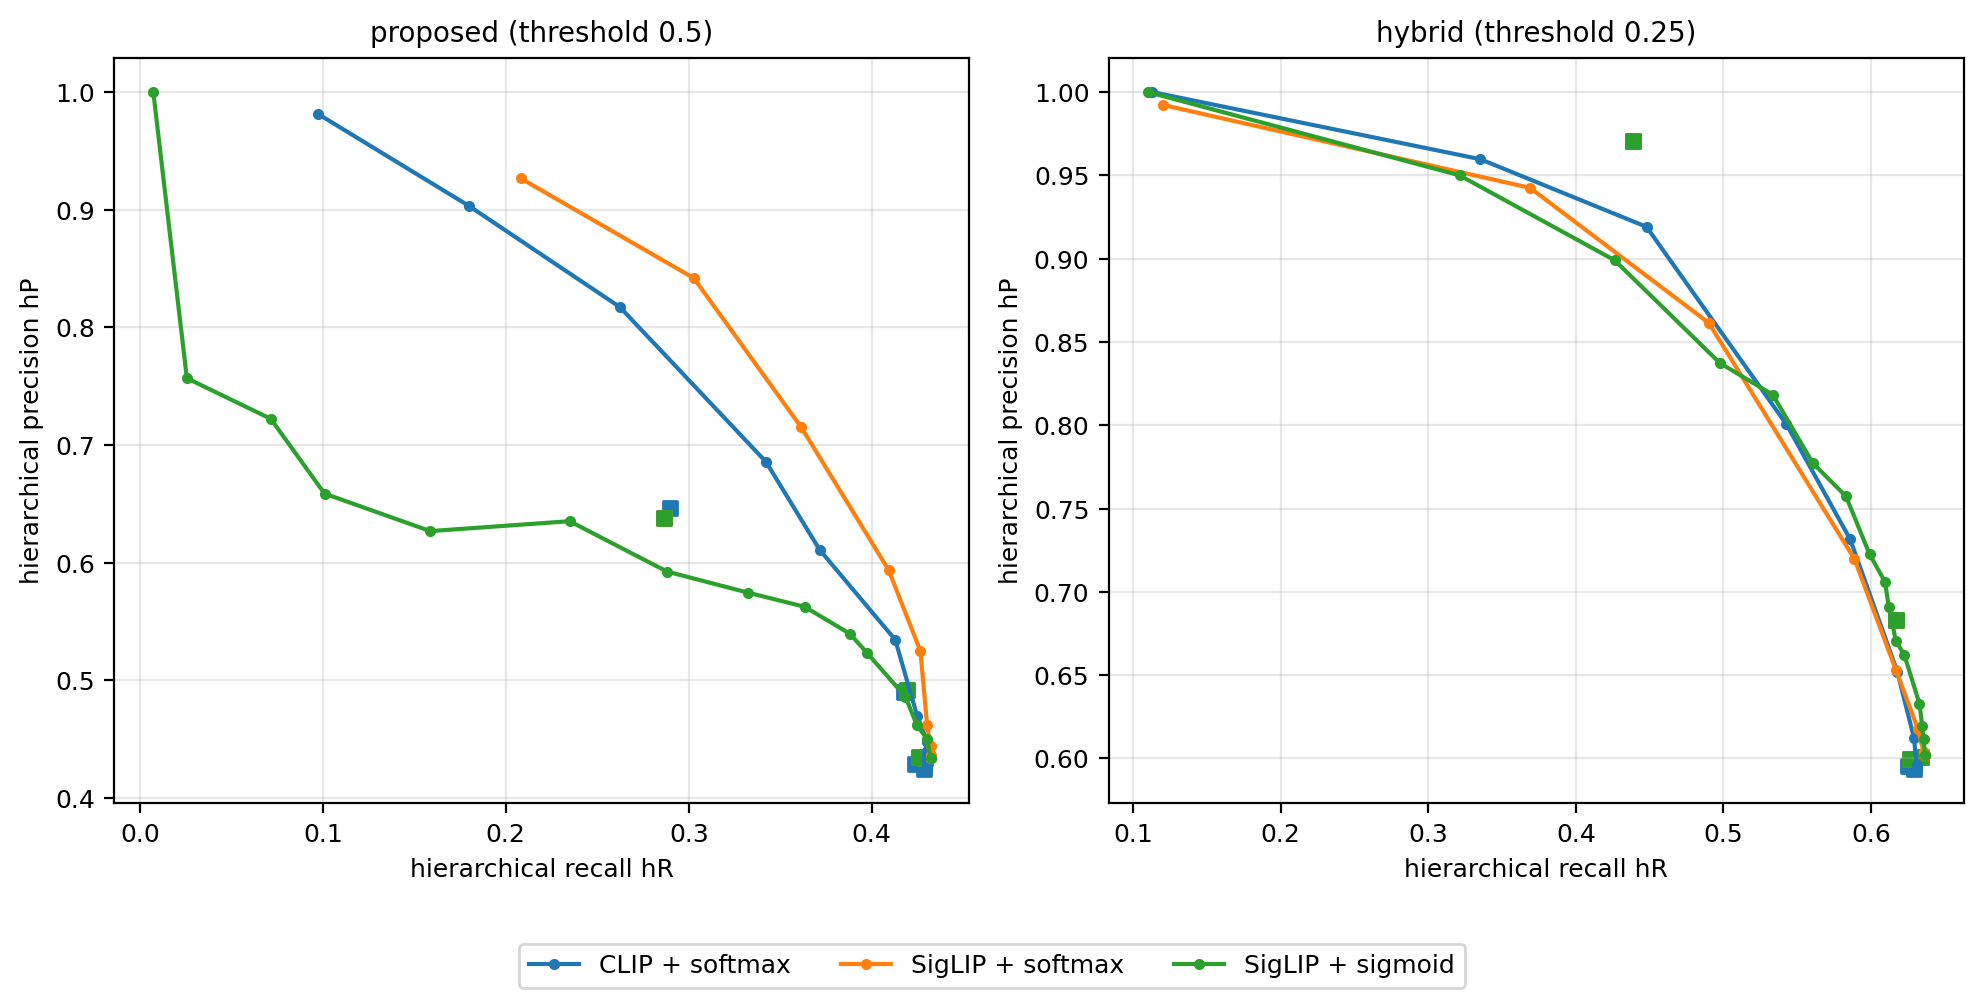
\includegraphics[width=\linewidth]{figures/fig_stopping_scorers.png}
    \caption{lvis\_testにおける階層的再現率$ hR $（横軸）と階層的適合率$ hP $（縦軸）の関係．曲線は累積確信度による停止規則，四角は深さの上限（0〜3）による停止規則である．}
    \label{fig_stopping_scorers}
\end{figure}

\subsection{YOLOとVLMのスコアの比較}
表\ref{tab_cmp}に，(\ref{eq_cmp})によるhybrid\_cmpのtest500の結果を示す．
切替はYOLOと異なる語が深さ0となったインスタンス数，改善と悪化はそれぞれYOLOの語が不正解でVLMの語が正解の数と，YOLOの語が正解でVLMの語が不正解の数である．

\begin{table}[t]
    \centering
    \caption{YOLOとVLMのスコアの比較による深さ0の決定（test500）．閾値はYOLO11xの検出スコアの閾値，Top-1の基準はYOLOの語をそのまま用いる場合のTop-1正解率である．}
    \label{tab_cmp}
    \small
    \setlength{\tabcolsep}{2.5pt}
    \begin{tabular}{clcccc}
        \toprule
        閾値 & VLMと正規化関数 & 切替 & 改善 & 悪化 & Top-1 \\
        \midrule
        \multirow{4}{*}{0.25} & 基準（hybrid） & -- & -- & -- & 0.969 \\
        & CLIP + ソフトマックス & 103 & 7 & 92 & 0.936 \\
        & SigLIP + ソフトマックス & 331 & 20 & 304 & 0.858 \\
        & SigLIP + シグモイド & 6 & 1 & 5 & 0.967 \\
        \midrule
        \multirow{4}{*}{0.7} & 基準（hybrid） & -- & -- & -- & 0.982 \\
        & CLIP + ソフトマックス & 21 & 0 & 21 & 0.969 \\
        & SigLIP + ソフトマックス & 127 & 5 & 122 & 0.908 \\
        & SigLIP + シグモイド & 1 & 0 & 1 & 0.982 \\
        \bottomrule
    \end{tabular}
\end{table}

表\ref{tab_cmp}から，ソフトマックスでは切替の大部分がYOLOの正解を不正解に変えており，Top-1正解率はCLIPで0.969から0.936へ，SigLIPで0.858へ低下した．
閾値0.25において，YOLOの検出スコアの中央値は0.787であるのに対し，VLMの最大確信度の中央値はCLIPとソフトマックスで0.391，SigLIPとソフトマックスで0.755，SigLIPとシグモイドで0.022であった．
VLMの最大確信度がYOLOの検出スコアを上回るインスタンスの割合は，それぞれ24.0\%，52.2\%，3.0\%であり，SigLIPとソフトマックスで切替が最も多い．
シグモイドではVLMの確信度がYOLOの検出スコアを上回ることがほとんどなく，切替は6件にとどまり，Top-1正解率はほぼ変わらなかった．
YOLOの検出スコアとVLMの確信度は異なるモデルの異なる尺度の値であり，(\ref{eq_cmp})の切替の頻度は，予測の正しさではなく両者の尺度の違いで決まる．
なお，$ {\mathbb V}_0 $がCOCOの80クラスであるhybrid\_cmpは，COCO外の物体に正しい上位語を与えることはできず，COCO外の物体の正解率はすべての組で0であった．

\subsection{WordNetの同じ深さの語彙}
表\ref{tab_wn_vocab}に(\ref{eq_wn_vocab})の語彙の統計を示す．
COCO外の22語のうち語彙に含まれるのは，$ k = 2 $でmonkey，deer，fox，squirrelの4語であった．
penguin，camel，kangaroo，helicopter等は，COCOのカテゴリのいとこより深い語であるため含まれない．
lvis\_testのCOCO外の511カテゴリのうち，語彙に上位語または自身を持つカテゴリは$ k = 2 $で232カテゴリ（45\%）である．

\begin{table}[t]
    \centering
    \caption{WordNetの同じ深さの語彙の統計．COCO外はCOCOの80クラス以外の語数，22語はCOCO外の22語のうち語彙に含まれる語数，LVISはlvis\_testのCOCO外の511カテゴリのうち語彙に上位語または自身を持つカテゴリ数である．}
    \label{tab_wn_vocab}
    \begin{tabular}{ccccc}
        \toprule
        $ k $ & 語彙数 & COCO外 & 22語 & LVIS \\
        \midrule
        1 & 213 & 133 & 2 & 96 \\
        2 & 681 & 601 & 4 & 232 \\
        3 & 1115 & 1035 & 5 & 289 \\
        \bottomrule
    \end{tabular}
\end{table}

図\ref{fig_tradeoff}に，深さ0の決め方ごとの，COCOのTop-1正解率とCOCO外の物体の正解率の関係を示す．
横軸はtest500の深さ0のTop-1正解率，縦軸はlvis\_testのCOCO外の物体のうち深さ0の語がLVISのSynsetの上位語または自身である割合であり，閾値はいずれも0.25である．

\begin{figure}[t]
    \centering
    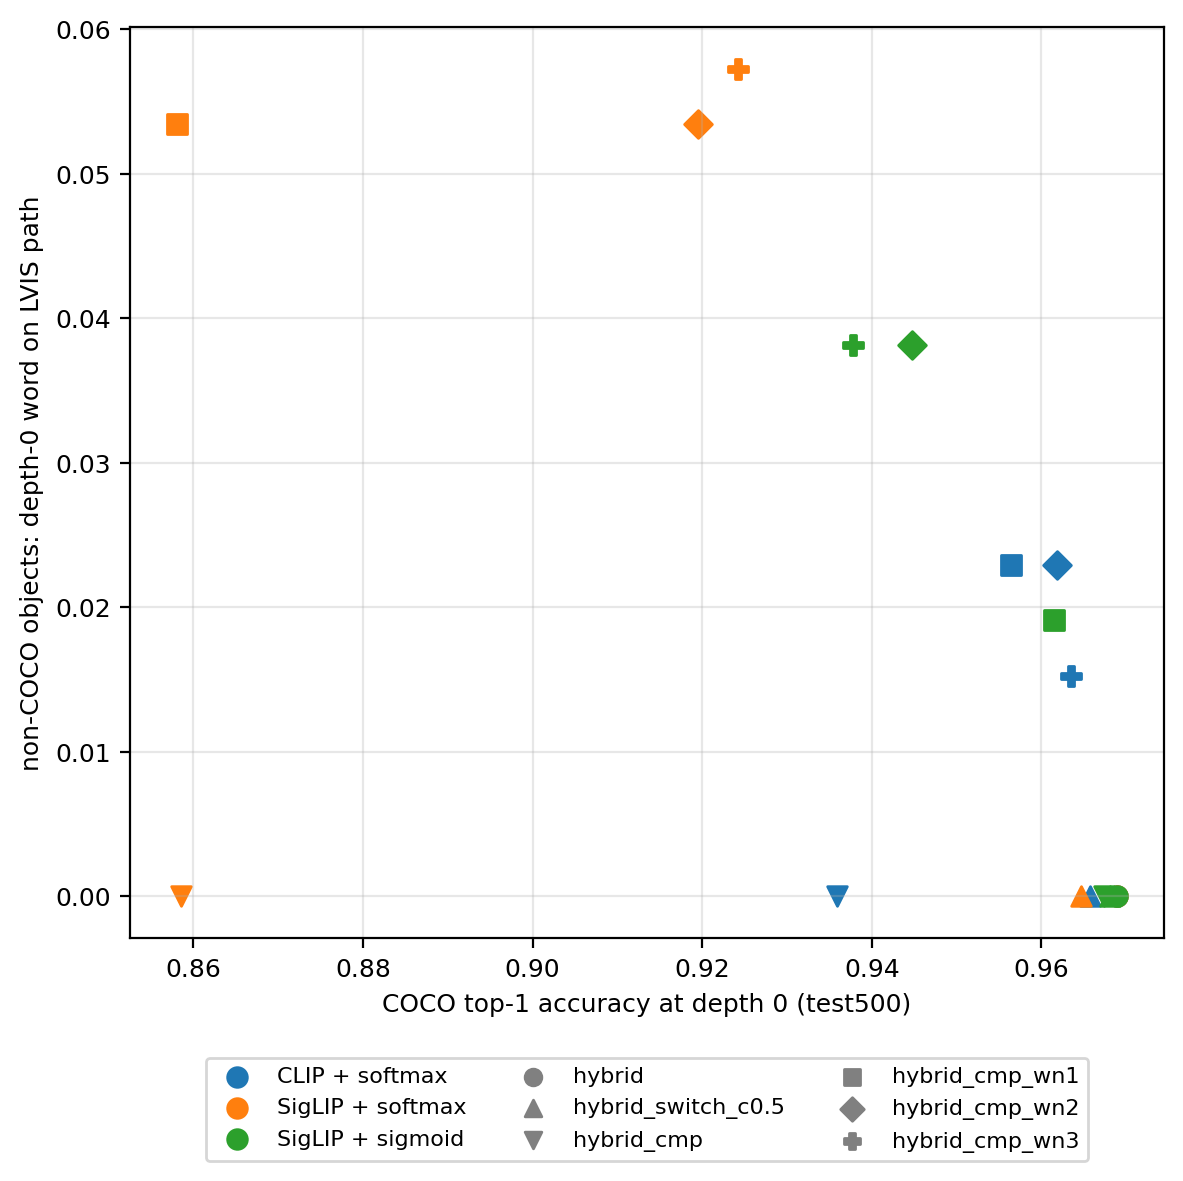
\includegraphics[width=0.9\linewidth]{figures/fig_tradeoff.png}
    \caption{COCOのTop-1正解率（横軸，test500）とCOCO外の物体の深さ0の正解率（縦軸，lvis\_test）の関係．色はVLMと正規化関数，形は深さ0の決め方を表し，YOLO11xの閾値は0.25である．}
    \label{fig_tradeoff}
\end{figure}

図\ref{fig_tradeoff}から，hybrid，hybrid\_switch\_c0.5およびhybrid\_cmpはCOCO外の物体の正解率が0である．
WordNetの同じ深さの語彙を用いたhybrid\_cmp\_wn2では，SigLIPとシグモイドでCOCO外の物体の正解率が3.8\%（262件中10件）に上がった一方，COCOのTop-1正解率は0.969から0.945へ低下した．
test500では65件がYOLOと異なる語に切り替わり，そのうち62件がYOLOの正解を不正解に変えた．
悪化の例は，personをleg，tvをscreen，ovenをstoveとするものであり，物体の部分や類義の語が選ばれている．
COCO外の物体で正しく命名できた例は，plate，can，pear，sack，pot，bucket等の容器や食品であった．
DETRに対して$ {\mathbb V}_0^{(2)} $から深さ0を選ぶproposed\_wn2では，COCO外の物体の正解率は10.0\%（SigLIP）であるが，COCOのTop-1正解率は0.527から0.304へ大きく低下した．
また，語彙には「slit」「worsted」「column」のように物体の名前として用いられにくい多義の語が含まれ，COCO外の物体の深さ0の上位にこれらの語が現れた．

図\ref{fig_qualitative}に，COCO外の物体の実画像に対する，SigLIPとシグモイドでの定性結果を示す．
上段の現在の構成（hybrid\_switch\_c0.5）では，penguinの3領域のうち2領域とcamelがCOCO外の語に切り替わった．
下段のhybrid\_cmp\_wn2では，penguinはbirdとなり，COCOと同じ深さの語としては正しい．
しかし，camelとkangarooは語彙に含まれないため，YOLOのdogとsheepのままであった．

\begin{figure*}[t]
    \centering
    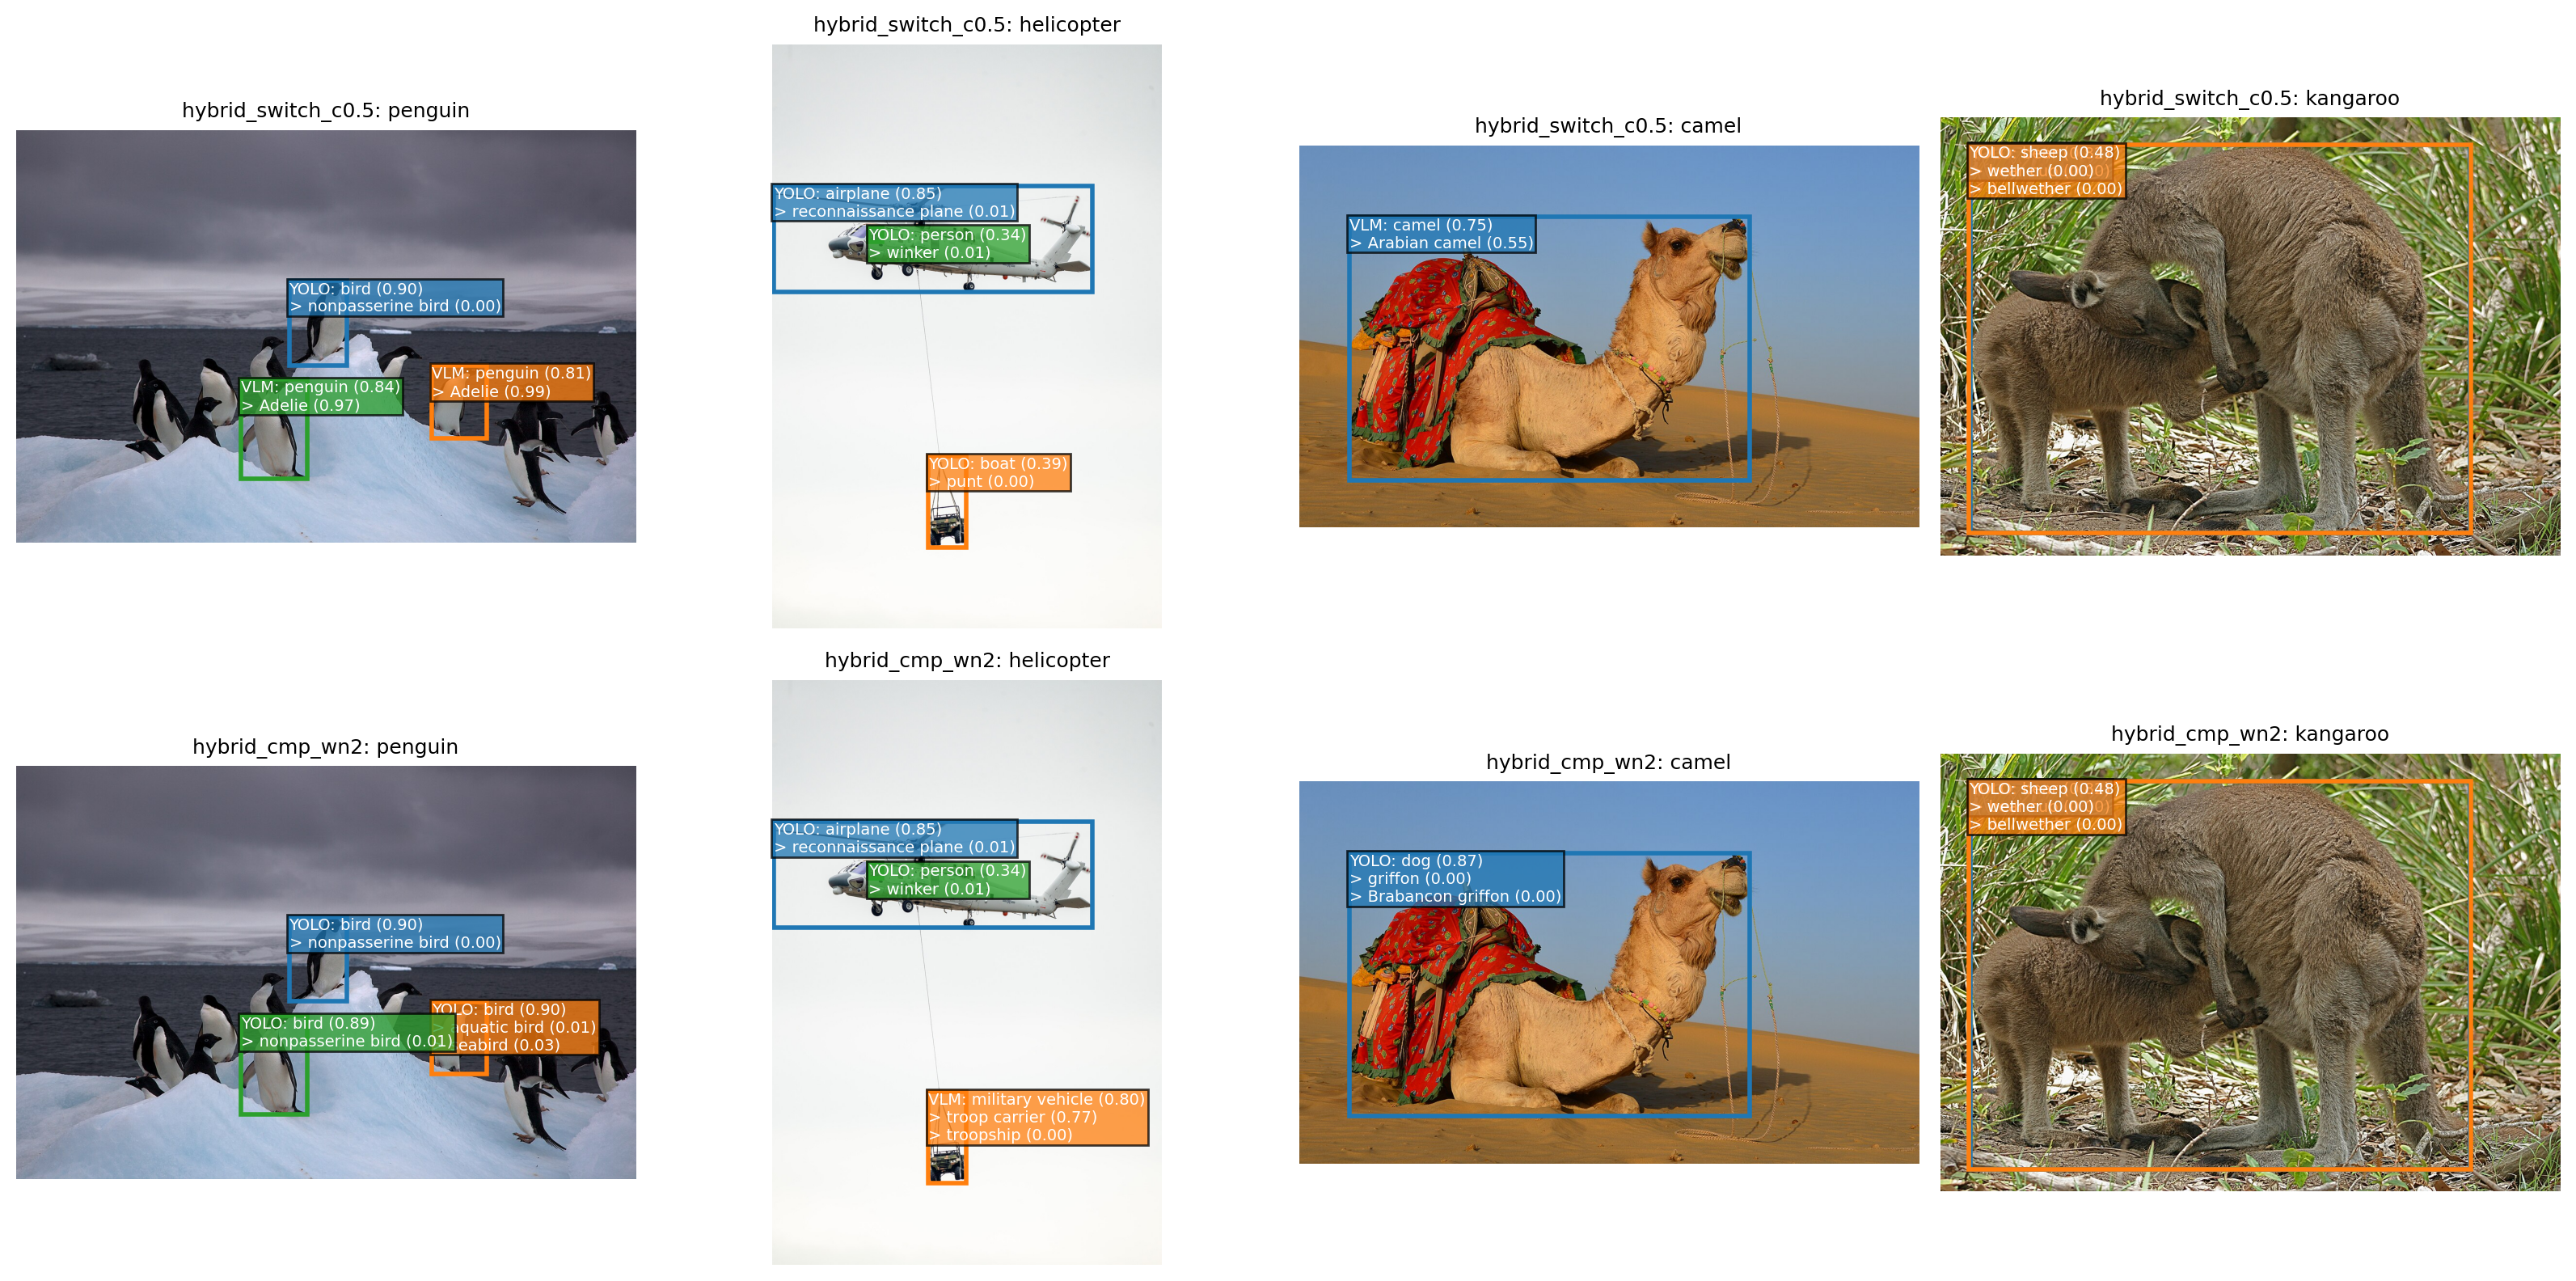
\includegraphics[width=0.85\linewidth]{figures/fig_qualitative.png}
    \caption{COCO外の物体の実画像に対する定性結果（SigLIPとシグモイド，YOLO11xの閾値0.25）．上段はCOCO外の22語への切替（hybrid\_switch\_c0.5），下段はWordNetの同じ深さの語彙とスコアの比較（hybrid\_cmp\_wn2）である．深さ0の語の前に，その決定に用いたモデルを``YOLO:''，``VLM:''で示す．画像はWikimedia Commons（CC BY 2.0，CC0，CC BY-SA 3.0/4.0）より取得した．}
    \label{fig_qualitative}
\end{figure*}

\section{考察}
\subsection{現在の構成との比較のまとめ}
表\ref{tab_summary}に，CLIPとソフトマックスを用いるhybridを基準とした3つの変更の効果をまとめる．
シグモイドへの変更は，深さ0の誤りを深い段階で検出できないという現在の構成の課題に対し，誤った枝の識別性能を改善する点で有効である．
一方，深さ0が正しい場合の深さ1の判断ではソフトマックスの方が識別性能が高く，停止規則の$ hF $の改善はhybridで0.012にとどまった．
両者の性質は相補的であり，各段階の語の選択と兄弟の語の間の比較にはソフトマックス，誤った枝の検出と棄却にはシグモイドを用いる組み合わせが考えられる．

\begin{table}[t]
    \centering
    \caption{CLIPとソフトマックスを用いるhybridを基準とした3つの変更の効果（テスト用の分割，YOLO11xの閾値0.25）．}
    \label{tab_summary}
    \small
    \setlength{\tabcolsep}{2pt}
    \begin{tabular}{lcc}
        \toprule
        変更 & 改善した指標 & 悪化した指標 \\
        \midrule
        シグモイド & \shortstack{誤枝AUROC \\ 0.418 → 0.617} & \shortstack{深さ1のAUROC \\ 0.762 → 0.644} \\
        \midrule
        スコアの比較 & -- & \shortstack{Top-1 0.969 → 0.936 \\（ソフトマックス）} \\
        \midrule
        \shortstack{WordNetの \\ 同じ深さの語彙} & \shortstack{COCO外の正解率 \\ 0 → 3.8\%} & \shortstack{Top-1 \\ 0.969 → 0.945} \\
        \bottomrule
    \end{tabular}
\end{table}

YOLOとVLMのスコアの比較は，尺度の異なる2つの値を直接比較するため，正規化関数を変えるだけで切替の頻度が6件から331件まで変化した．
2つのモデルのスコアを比較するためには，検証用の分割で各モデルの確信度を正解率に対応付ける較正を行った上で比較する必要がある．

WordNetの同じ深さの語彙は，COCOと同じ粒度の語でCOCO外の物体を命名するという目的には合致するが，現在の語彙では効果が小さい．
第一の理由は，表\ref{tab_wn_vocab}から，lvis\_testのCOCO外の物体のカテゴリの半数以上が語彙に上位語または自身を持たないことである．
第二の理由は，WordNetのレンマには物体の部分（leg，screen）や多義の語（slit，worsted）が含まれ，VLMがこれらを選ぶとCOCOの物体の正解が失われることである．
また，同じ深さの制約により，penguinやcamelのように直観的には基本的な語であってもCOCOのいとこより深い語は語彙から除かれる．
WordNetの深さと人が用いる名前の粒度は一致しないため，具体性の評定や画像データセットでの出現頻度等，物体の名前としての用いられやすさを考慮した語彙の選択が必要である．

\subsection{論文への反映}
論文の主張に対し，シグモイドの結果は，深い段階の確信度が誤りの手がかりにならないという課題に対する有効な対策として追記できる．
スコアの比較とWordNetの同じ深さの語彙は，現在の結果ではhybrid\_switch\_c0.5を上回らないため，提案手法として採用するのではなく，COCO外の語彙への体系的な拡張の検討結果と今後の課題として記述するのが妥当である．

\section{おわりに}
本稿では，検出と命名を分離した粒度可変物体アノテーションに対し，SigLIPとシグモイドによる確信度，YOLOとVLMのスコアの比較による深さ0の決定，およびWordNetにおいてCOCOのカテゴリと同じ深さにある語彙を深さ0の候補とする3つの変更を，現在の構成と比較した．
シグモイドは，深さ0が誤った枝の識別性能をハイブリッド構成で0.418から0.617へ改善したが，深さ1の正誤の識別ではソフトマックスに劣った．
スコアの比較による切替は，YOLOとVLMの尺度の違いにより切替の頻度が大きく変わり，ソフトマックスではCOCOの精度を低下させた．
WordNetの同じ深さの語彙は，COCO外の物体の深さ0の正解率を3.8\%に上げる一方，COCOのTop-1正解率を0.945へ低下させた．
今後の課題として，ソフトマックスとシグモイドを組み合わせた確信度，YOLOとVLMの確信度の較正，および物体の名前としての用いられやすさを考慮した深さ0の語彙の選択が挙げられる．

\vspace{-1mm}
\begin{thebibliography}{99}

    \bibitem{ref_DETR}
    N. Carion, F. Massa, G. Synnaeve, N. Usunier, A. Kirillov, and S. Zagoruyko,
    ``End-to-End Object Detection with Transformers,''
    in {\it Proc. European Conference on Computer Vision (ECCV)}, 2020.

    \bibitem{ref_YOLO}
    J. Redmon, S. Divvala, R. Girshick, and A. Farhadi,
    ``You Only Look Once: Unified, Real-Time Object Detection,''
    in {\it Proc. IEEE Conference on Computer Vision and Pattern Recognition (CVPR)}, 2016.

    \bibitem{ref_CLIP}
    A. Radford, J. W. Kim, C. Hallacy, A. Ramesh, G. Goh, S. Agarwal, G. Sastry, A. Askell, P. Mishkin, J. Clark, G. Krueger, and I. Sutskever,
    ``Learning Transferable Visual Models From Natural Language Supervision,''
    in {\it Proc. International Conference on Machine Learning (ICML)}, 2021.

    \bibitem{ref_WordNet}
    G. A. Miller,
    ``WordNet: A Lexical Database for English,''
    {\it Communications of the ACM}, vol. 38, no. 11, pp. 39--41, 1995.

    \bibitem{ref_COCO}
    T.-Y. Lin, M. Maire, S. Belongie, J. Hays, P. Perona, D. Ramanan, P. Doll\'{a}r, and C. L. Zitnick,
    ``Microsoft COCO: Common Objects in Context,''
    in {\it Proc. European Conference on Computer Vision (ECCV)}, 2014.

    \bibitem{ref_SigLIP}
    X. Zhai, B. Mustafa, A. Kolesnikov, and L. Beyer,
    ``Sigmoid Loss for Language Image Pre-Training,''
    in {\it Proc. IEEE/CVF International Conference on Computer Vision (ICCV)}, pp. 11975--11986, 2023.

    \bibitem{ref_SemCor}
    G. A. Miller, C. Leacock, R. Tengi, and R. T. Bunker,
    ``A Semantic Concordance,''
    in {\it Proc. ARPA Workshop on Human Language Technology}, pp. 303--308, 1993.

    \bibitem{ref_LVIS}
    A. Gupta, P. Doll\'{a}r, and R. Girshick,
    ``LVIS: A Dataset for Large Vocabulary Instance Segmentation,''
    in {\it Proc. IEEE/CVF Conference on Computer Vision and Pattern Recognition (CVPR)}, pp. 5356--5364, 2019.

    \bibitem{ref_hF}
    S. Kiritchenko, S. Matwin, R. Nock, and A. F. Famili,
    ``Learning and Evaluation in the Presence of Class Hierarchies: Application to Text Categorization,''
    in {\it Proc. Canadian Conference on Artificial Intelligence}, pp. 395--406, 2006.

\end{thebibliography}


\end{document}
